\documentclass{osa-article}

%% Select the journal you're submitting to
%% oe, boe, ome, osac, osajournal
\journal{osajournal}
% Key:
% Express journals must have the correct journal selected:
% {oe} Optics Express
% {boe} Biomedical Optics Express
% {ome} Optical Material Express
% {osac} OSAC Continuum
% Other OSA journals may use:
% {osajournal} Applied Optics, Advances in Optics and Photonics, Journal of the Optical Society of America A/B, Optics Letters, Optica, Photonics Research

% Uncomment if submitting to Photonics Research.
% ONLY APPLICABLE FOR \journal{osajournal}
% \setprjcopyright

% Set the article type
\articletype{Research Article}
% Note that article type is not required for Express journals (OE, BOE, OME and OSAC)

% Talon's custom commands
\newcommand{\argmin}{\arg\!\min}
\newcommand{\me}{\mathrm{e}}
\providecommand{\e}[1]{\ensuremath{\times 10^{#1}}} 
\providecommand{\mb}[1]{\mathbf{#1}}
\providecommand{\mf}[1]{\mathfrak{#1}}
\providecommand{\mc}[1]{\mathcal{#1}}
\providecommand{\ro}[1]{\mathbf{\mathbf{r}}_o}
\providecommand{\so}[1]{\mathbf{\hat{s}}_o}
\providecommand{\rb}[1]{\mathbf{r}_b}
\providecommand{\rbm}[1]{r_b^{\text{m}}}
\providecommand{\rd}[1]{\mathbf{r}_d}
\providecommand{\rdf}{\mathpzc{r}_d}
\providecommand{\mh}[1]{\mathbf{\hat{#1}}}
\providecommand{\mbb}[1]{\mathbb{#1}}
\providecommand{\bs}[1]{\boldsymbol{#1}}
\providecommand{\bsh}[1]{\hat{\boldsymbol{#1}}}
\providecommand{\nan}{\left(\frac{\text{NA}}{n_o}\right)}
\DeclareFontFamily{OT1}{pzc}{}
\DeclareFontShape{OT1}{pzc}{m}{it}{<-> s * [1.10] pzcmi7t}{}
\DeclareMathAlphabet{\mathpzc}{OT1}{pzc}{m}{it}

\begin{document}

\title{Spatio-angular transfer functions for fluorescence microscopes I. Basic theory}

\author{Talon Chandler,\authormark{1,*} Author order TBD,\authormark{2,*} and Patrick La Rivi\`ere \authormark{1}}

\address{\authormark{1}University of Chicago, Department of Radiology, Chicago, Illinois 60637, USA\\
\authormark{2}Publications Department, The Optical Society, 2010 Massachusetts Avenue NW, Washington, DC 20036, USA\\
\authormark{3}Currently with the Department of Electronic Journals, The Optical Society, 2010 Massachusetts Avenue NW, Washington, DC 20036, USA}

\email{\authormark{*}talonchandler@talonchandler.com} %% email address is required

%\homepage{talonchandler@talonchandler.com} %% author's URL, if desired

%%%%%%%%%%%%%%%%%%% abstract %%%%%%%%%%%%%%%%
%% [use \begin{abstract*}...\end{abstract*} if exempt from copyright]

\begin{abstract*}
  We introduce the basic elements of a complete spatio-angular theory of
  fluorescence microscopes. We start by analyzing a single-view fluorescence
  microscope imaging an ensemble of in-focus dipole absorber/emitters using
  electromagnetic optics and the paraxial approximation. Next, we define the
  spatio-angular transfer function and show that fluorescence microscopes have
  an angular band limit. Finally, we discuss the implications of our analysis on
  quantitative fluorescence microscopy studies.
\end{abstract*}

%%%%%%%%%%%%%%%%%%%%%%%%%%  body  %%%%%%%%%%%%%%%%%%%%%%%%%%
\section{Introduction}
Fluorescence microscopes are ubiquitous tools in biology [XXX], materials
science [XXX], and metrology [XXX] for measuring the concentration of
fluorophores throughout a sample. While an unprocessed fluorescence micrograph
reports the approximate concentration of fluorophores throughout a sample,
diffraction-limited microscopes image a spatially blurred version of the true
fluorophore distribution. Therefore, microscopists who are interested in
accurate measurements will perform a computational restoration to recover some
of the information lost during the imaging process.

Restoration techniques attempt to recover the true distribution of fluorophores
using the measured data and a model of the imaging process. The model of the
imaging process can be obtained theoretically (by mathematically modeling the
instrument under idealized conditions), experimentally (by measuring the
microscope's response to a known input), or by a combination of theory and
experiment (by measuring parameters of an instrument model). In all cases, the
accuracy of the restored image is limited by the accuracy of the imaging model.

Most theoretical fluorescence microscopy imaging models make simplifying
approximations. A common (often unstated) pair of approximations is to (1) treat
fluorophores as monopole absorber/emitters and (2) treat light propagation under
the scalar approximation. In this work we will analyze fluorescence microscopes
without these approximations and find the conditions under which these
approximations are valid.

Using an experimentally determined model is an effective way to find an accurate
model without understanding all of the physical details of the imaging system,
but these approaches require a known input that can completely characterize the
imaging system. Sub-diffraction beads are commonly used as a known input for
measuring the response of a microscope, but we argue that sub-diffraction beads
are not enough to completely characterize the response of a microscope to all
fluorescent samples. Beads can only characterize the response of the microscope
to an angularly uniform distribution of fluorophores, and we will show that all
microscopes have an orientation-dependent response. A complete characterization
requires a test sample with at least three known orientation distributions.

The single-molecule localization microscopy (SMLM) community has pioneered the
use of rigorous electromagnetic models of single fluorescence microscopes
\cite{backer2014, lieb2004}. When only one fluorophore is emitting at a time,
the measured intensity pattern is strongly dependent on the orientation of the
emitting molecule. Backlund and Lew \cite{backlund2014} have shown that ignoring
the orientation of fluorophores can lead to biased estimates of their position,
so the most accurate SMLM experiments must jointly estimate the position and
orientation of the molecule. These joint estimates usually use a set of
precomputed intensity patterns and a maximum-likelihood algorithm to estimate
the orientation and position of each molecule. These methods have led to some of
the most accurate position estimates of single molecules.

Meanwhile, most fluorescence microscopists image ensembles of fluorophores.
Although many groups have used polarizers to probe the orientation of ensembles
of fluorophores \cite{mehta2016} [Forkey], to our knowledge no
work has been done on the response of fluorescence microscopes to ensembles of
oriented fluorophores. Furthermore, current restoration techniques in polarized
light microscopy are lacking because they rely on simple pixel-wise arithmetic
and do not model the propagation of light through the microscope.

In this work we model ensembles of in-focus dipole absorber/emitters using
electromagnetic optics and the paraxial approximation. This marks a first step
towards a complete three-dimensional non-paraxial theory of fluorescence
microscopes. In section 2 we model the excitation and detection processes of
dipoles. We define the most important quantity in this work, the spatio-angular
transfer function, and we use it to show that fluorescence microscopes have an
angular band limit. In section 3 we perform simulations and compare our model to
traditional scalar models. In section 4 we discuss the implications of our work
for fluorescence microscopy and lay out a path towards a complete spatio-angular
theory of fluorescence microscopy.

\section{Theory}
\subsection{Spherical harmonics}\label{sec:sph}
\begin{align}
  y_l^m(\vartheta, \varphi) =
  \begin{cases}
    \sqrt{2}K_l^m\cos(m\varphi)P_l^m(\cos\vartheta), & m > 0\\
    K_l^0P_l^0(\cos\vartheta), & m = 0\\
    \sqrt{2}K_l^m\sin(-m\varphi)P_l^{-m}(\cos\vartheta), & m < 0\\
  \end{cases}
\end{align}
where
\begin{align}
  K_l^m = \sqrt{\frac{(2l+1)}{4\pi}\frac{(l-|m|)!}{(l+|m|)!}},
\end{align}
and $P_l^m(x)$ are the associated Legendre polynomials. The $l=0, 1, 2$
spherical harmonics are given by
\begin{align}
  y_0^0(\vartheta, \varphi) &= \sqrt{\frac{1}{4\pi}}, \nonumber \\ 
  y_1^{-1}(\vartheta, \varphi) = \sqrt{\frac{3}{4\pi}}\sin\varphi\sin\vartheta, \hspace{2em} y_1^0(\vartheta, \varphi) &= \sqrt{\frac{3}{4\pi}}\cos\vartheta, \hspace{2em} y_1^1(\vartheta, \varphi) = \sqrt{\frac{3}{4\pi}}\cos\varphi\sin\vartheta, \nonumber \\
  y_2^{-2}(\vartheta, \varphi) = \sqrt{\frac{15}{4\pi}}\sin\varphi\cos\varphi\sin^2\vartheta, &\hspace{2em} y_2^{-1}(\vartheta, \varphi) = \sqrt{\frac{15}{4\pi}}\sin\varphi\sin\vartheta\cos\vartheta,\nonumber \\
  y_2^0(\vartheta, \varphi) &= \sqrt{\frac{5}{16\pi}}(3\cos^2\vartheta - 1), \nonumber \\ 
  y_2^{1}(\vartheta, \varphi) = \sqrt{\frac{15}{4\pi}}\cos\varphi\sin\vartheta\cos\vartheta, &\hspace{2em} y_2^{2}(\vartheta, \varphi) = \sqrt{\frac{15}{4\pi}}(\cos^2\varphi - \sin^2\varphi)\sin^2\vartheta.\label{eq:harmonics}
\end{align}

\subsection{Excitation model}
% [theta**2*cos(phi - phip)**2/2 + 0.5*sin(phip)**2 + 0.5*cos(phip)**2, 0, 0, 0, sqrt(15)*sin(2*phip)/10, -sqrt(15)*theta*sin(phip)*cos(phi - phip)/5, sqrt(5)*theta**2*cos(phi - phip)**2/5 - sqrt(5)*sin(phip)**2/10 - sqrt(5)*cos(phip)**2/10, -sqrt(15)*theta*cos(phip)*cos(phi - phip)/5, -sqrt(15)*sin(phip)**2/10 + sqrt(15)*cos(phip)**2/10]
In this section we will calculate the excitation kernel for epi-illumination
microscopes---the relative probability of exciting a molecule with a known
orientation. Our approach is similar to previous work \cite{fourkas2001,  chandler2017},
but here we consider unpolarized illumination and restrict
ourselves to the paraxial approximation.

We consider a single molecule with a fixed absorption dipole moment $\so{}$ that
we express in spherical coordinates [see Fig. 1(a)] as 
\begin{align}
  \so{} &= \cos\varphi\sin\vartheta\mh{x} + \sin\varphi\sin\vartheta\mh{y} + \cos\vartheta\mh{z}. \label{eq:spherical}
\end{align}
We can rewrite Eq. \ref{eq:spherical} in terms of spherical harmonic functions
(see Section \ref{sec:sph}) as
\begin{align}
  \so{} &=\sqrt{\frac{3}{4\pi}}\left[y_1^1(\vartheta, \varphi)\,\mh{x} + y_1^{-1}(\vartheta, \varphi)\,\mh{y} + y_1^0(\vartheta, \varphi)\, \mh{z}\right]. \label{eq:sphharm}
\end{align}
We place the molecule in the focal plane of an aplanatic and
polarization-preserving objective lens with its optical axis aligned with the
$\mh{z}$ axis. Next, we place a spatially incoherent, spatially uniform,
unpolarized thermal light source (or its image) in the back aperture of the
objective lens to illuminate the focal plane. In this geometry each point in the
back focal plane generates a plane wave that illuminates the sample.

To model the unpolarized light source we will use polarized ray tracing [cite
Torok] to find the response for a single polarized ray, then integrate over the
rays and polarizations to find the complete response. First, we model the
electric field at every point on the back focal plane as
\begin{align}
   \mb{E}_{\text{bfp}}(\phi_{\text{pol}}) &\propto \cos\phi_{\text{pol}}\mh{x} + \sin\phi_{\text{pol}}\mh{y}, \label{eq:bfp0}
\end{align}
where $\phi_{\text{pol}}$ is the polarization orientation and \{$\mh{x}$,
$\mh{y}$\} are transverse Cartesian basis vectors. Notice that Eq. \ref{eq:bfp0}
describes the incoherent electric fields at every point in the back focal plane,
it does not describe a coherent plane wave. Immediately after the lens the
electric field is
\begin{align}
  \mb{E}_{\text{ff}}(\theta, \phi, \phi_{\text{pol}}) \propto \left\{[\mb{E}_\text{bfp}(\phi_{\text{pol}})\cdot\bsh{\phi}]\,\bsh{\phi} + [\mb{E}_\text{bfp}(\phi_{\text{pol}})\cdot\bsh{\rho}]\,\bsh{\theta}\right\}\sqrt{\cos\theta}, \label{eq:bfp2ff}
\end{align}
where \{$\theta$, $\phi$\} are spherical coordinates, \{$\bsh{\rho}$,
$\bsh{\phi}$\} are cylindrical basis vectors, and \{$\bsh{\theta}$,
$\bsh{\phi}$\} are spherical basis vectors defined in Figure 1(a) and related by
\begin{align}
  \bsh{\rho} &= \cos\phi\mh{x} + \sin\phi\mh{y},\label{eq:rho}\\
  \bsh{\phi} &= -\sin\phi\mh{x} + \cos\phi\mh{y},\label{eq:phi}\\
  \bsh{\theta} &= \cos\phi\cos\theta\mh{x} + \sin\phi\cos\theta\mh{y} - \sin\theta\mh{z}.\label{eq:theta}               
\end{align}
In Eq. \ref{eq:bfp2ff} the
$[\mb{E}_\text{bfp}(\phi_{\text{pol}})\cdot\bsh{\phi}]\,\bsh{\phi}$ term models
s-polarized fields, the
$[\mb{E}_\text{bfp}(\phi_{\text{pol}})\cdot\bsh{\rho}]\,\bsh{\theta}$ term
models the rotation of p-polarized fields, and the $\sqrt{\cos\theta}$ term
models the apodization of an aplanatic lens. After plugging Eq. \ref{eq:bfp0}
and Eqs. \ref{eq:rho}--\ref{eq:theta} into Eq. \ref{eq:bfp2ff} and applying the
paraxial approximation, the electric field immediately after the lens is given
by
\begin{align}
  \mb{E}_{\text{ff}}^{(p)}(\theta, \phi, \phi_{\text{pol}}) \propto \cos\phi_{\text{pol}}\mh{x} + \sin\phi_{\text{pol}}\mh{y} - \theta\cos(\phi - \phi_{\text{pol}})\mh{z}.\label{eq:eff}
\end{align}
To calculate the probability that a dipole oriented along $\so{}$ is excited by
a ray with electric field $\mb{E}$ we need to evaluate $|\mb{E}\cdot\so{}|^2$.
Evaluating this expression for each ray would be cumbersome if we used Eqs.
\ref{eq:spherical} and \ref{eq:eff} because we would need to simplify a large
number of trigonometric functions. Instead, we use Eqs. \ref{eq:sphharm} and
\ref{eq:eff} and the real Gaunt coefficients [XXXciteXXX] to find the products
of spherical harmonics. We find that
% [theta**2*cos(phi - phip)**2/2 + 0.5*sin(phip)**2 + 0.5*cos(phip)**2, 0, 0, 0, sqrt(15)*sin(2*phip)/10, -sqrt(15)*theta*sin(phip)*cos(phi - phip)/5, sqrt(5)*theta**2*cos(phi - phip)**2/5 - sqrt(5)*sin(phip)**2/10 - sqrt(5)*cos(phip)**2/10, -sqrt(15)*theta*cos(phip)*cos(phi - phip)/5, -sqrt(15)*sin(phip)**2/10 + sqrt(15)*cos(phip)**2/10]
\begin{align}
  |\mb{E}_{\text{ff}}^{(p)}(\theta, \phi, \phi_{\text{pol}}) \cdot \so{}|^2 \propto\, &\left[1 + \theta^2\cos^2(\phi - \phi_{\text{pol}})\right]y_0^0(\so{}) + \frac{1}{\sqrt{5}}\left[ - 1 + 2\theta^2\cos^2(\phi - \phi_{\text{pol}})\right]y_2^{0}(\so{}) +\nonumber \\
                                   &\frac{\sqrt{15}}{10}\theta\sin\phi_{\text{pol}}\cos(\phi - \phi_{\text{pol}})y_2^{-1}(\so{}) + \frac{\sqrt{15}}{10}\theta\cos\phi_{\text{pol}}\cos(\phi - \phi_{\text{pol}})y_2^{1}(\so{}) -\nonumber \\  
                                   &\frac{\sqrt{15}}{20}\sin(2\phi_{\text{pol}})y_2^{-2}(\so{}) - \frac{\sqrt{15}}{20}\cos(2\phi_{\text{pol}})y_2^{2}(\so{}).\label{eq:integrand}
\end{align}
To calculate the complete excitation model we need to integrate Eq.
\ref{eq:integrand} over all polarization orientations and rays
\begin{align}
  h_{\text{exc}}(\so{}) \propto \int_0^{\alpha}\theta d\theta\int_0^{2\pi}d\phi\int_0^{2\pi}d\phi_{\text{pol}}\, |\mb{E}_{\text{ff}}^{(p)} \cdot \so{}|^2. \label{eq:integral}
\end{align}
After plugging Eq. \ref{eq:integrand} into Eq. \ref{eq:integral} and evaluating
the integrals, all but two terms disappear and the orientation-dependent
excitation model is given by
\begin{align}
  h_{\text{exc}}(\so{}) &\propto \left[1 + \frac{\alpha^2}{4}\right]y_0^0(\so{}) + \frac{1}{\sqrt{5}}\left[-1 + \frac{\alpha^2}{2}\right]y_2^0(\so{}). \label{eq:excitation}
\end{align}
We note that the excitation model depends on the orientation of the molecule,
but it does not depend on the position of the molecule in the focal plane. This
is a direct consequence of our illumination geometry---we have placed incoherent
light sources in the back focal plane of the objective so each point in the
focal plane within the field of view is illuminated equally.

\subsection{Detection model}
In this section we will calculate the detection kernel of an epi-detection
microscope---the irradiance on the detector due to single molecule at a known
position with known orientation. Our approach is similar to \cite{backer2014,
  nov2006, agrawal2012}, but here we restrict ourselves to the paraxial
approximation.

We consider a single dipole emitter at the origin with a fixed dipole emission
moment oriented along $\so{}$---parallel to the excitation moment. The electric
field at a position $\mb{r}$ far from the dipole is given by
\begin{align}
  \mb{E}_{\text{ff}}(\mb{r}, \so{}) \propto \mh{r} \times \so{} \times \mh{r}. \label{eq:ff}
\end{align}
If we place the molecule in the focal plane of an aplanatic and
polarization-preserving objective lens with its optical axis aligned with the
$\mh{z}$ axis (or reuse the illumination objective), then the electric field in
the back focal plane of the lens is given by
\begin{align}
  \mb{E}_{\text{bfp}}(\rb{}, \so{}) \propto \left\{[\mb{E}_\text{ff}(\mb{r}, \so{})\cdot\bsh{\phi}]\,\bsh{\phi} + [\mb{E}_\text{ff}(\mb{r}, \so{})\cdot\bsh{\theta}]\,\bsh{\rho}\right\}\sqrt{1/\cos\theta}\,\Pi\left(\frac{r_b}{\sin\alpha}\right). \label{eq:bfp}
\end{align}
where the first term accounts for s-polarized fields, the second term accounts
for p-polarized fields, $\sqrt{1/\cos\theta}$ is the apodization factor for an
aplanatic lens, and
\begin{align}
  \Pi\left(\frac{r_b}{\sin\alpha}\right) =
  \begin{cases}
    1\quad \text{if}\quad r_b < \sin^{-1}\alpha,\\
    0\quad \text{else},
  \end{cases}
\end{align}
is the aperture stop. After expanding the dot products, applying the paraxial
approximation, and writing the dipole orientation $\so{}$ in terms of spherical
harmonic functions, we find that the electric field in the back focal plane is
given by
\begin{align}
  \mb{E}_{\text{bfp}}^{(p)}(\rb{}, \so{}) \propto \left\{\left[y_1^1(\so{}) - r_b\cos\phi_b y_1^0(\so{})\right]\mh{x} + \left[y_1^{-1}(\so{}) - r_b\sin\phi_b y_1^0(\so{})\right]\mh{y}\right\}\Pi\left(\frac{r_b}{\alpha}\right). \label{eq:bfp2}
\end{align}
We note that Eq. \ref{eq:bfp2} is identical to previously derived models
[Piestun, Backer] except here we have used the paraxial approximation and used
spherical harmonic functions.

Next we place a tube lens one focal length from the back focal plane and a
detector (see Figure XX)). Under the paraxial approximation we can find the
electric field in the detector plane by taking the Fourier transform of the
field in the back focal plane [Goodman]
\begin{align}
  \mb{E}_{\text{det}}^{(p)}(\rd{}, \so{}) &= \int_{\mbb{R}^2}d\rb{} \mb{E}_{\text{bfp}}^{(p)}(\rb{})\, \text{exp}\left[ik\,\rb{}\cdot\rd{}\right].\label{eq:det1}
\end{align}
To evaluate the integral we rewrite it in polar coordinates
\begin{align}
\mb{E}_{\text{det}}^{(p)}(\rd{}, \so{}) &= \int_{0}^{\alpha}r_bdr_b\int_0^{2\pi} d\phi_b\, \mb{E}_{\text{bfp}}^{(p)}(r_b, \phi_b)\, \text{exp}\left[ikr_b r_d\cos(\phi_b - \phi_d)\right],
\end{align}
substitute Eq. \ref{eq:bfp2}, and apply the following identities
\begin{align}
  \int_0^{2\pi}d\phi_b
  \left\{\substack{
    \sin(n\phi_b)\\
    \cos(n\phi_b)
  }\right\}
  \text{exp}\left[ikr_br_d\cos(\phi_b - \phi_d)\right] &= 2\pi i^n
  \left\{\substack{
    \sin(n\phi'_o)\\
    \cos(n\phi'_o)
  }\right\}J_n(k r_br_d),
  \end{align}
  \begin{align}
  \int_0^{\alpha} dr_b (r_b)^{n+1}J_{n}(kr_br_d) &= \alpha^{n+1}\left[\frac{J_{n+1}(k\alpha r_d)}{k r_d}\right],
  \end{align}
to find that 
\begin{align}
  \mb{E}_{\text{det}}^{(p)}(\rd{}, \so{}) \propto &\left[\frac{J_1(k\alpha r_d)}{k\alpha r_d}y_1^1(\so{}) - i\alpha \frac{J_2(k\alpha r_d)}{k\alpha r_d}\cos\phi_d y_1^0(\so{})\right]\mh{x}\, + \nonumber \\& \left[\frac{J_1(k\alpha r_d)}{k\alpha r_d}y_1^{-1}(\so{}) - i\alpha \frac{J_2(k\alpha r_d)}{k\alpha r_d}\sin\phi_d y_1^0(\so{})\right]\mh{y}.
\end{align}
We can find the irradiance on the detector by taking the modulus squared of the
electric field
\begin{align}
  h_{\text{det}}(\rd{}, \so{}) &\propto |\mb{E}_{\text{det}}^{(p)}(\rd{}, \so{})|^2.
\end{align}
We use the real Gaunt coefficients to find that
\begin{align}
h_{\text{det}}(\rd{}, \so{}) &\propto \left[a_1( r_d) + \frac{\alpha^2}{4} a_2( r_d)\right]y_0^0(\so{}) + \frac{1}{\sqrt{5}}\left[- a_1( r_d) + \frac{\alpha^2}{2} a_2( r_d)\right]y_2^0(\so{}), \label{eq:detection}
\end{align}
where we have defined
\begin{align}
  a_n(r_d) \equiv \frac{n}{\pi}\left[\frac{J_n(k\alpha r_d)}{k\alpha r_d}\right]^2. 
\end{align}

In our analysis we have only considered a dipole radiator at the origin, but we
can use the shift-invariance of 4$f$ imaging systems to model dipole radiators
at arbitrary positions in the focal plane. If we shift the dipole radiator to an
in-focus position $\ro{}$, then the irradiance pattern on the detector will be
given by $h_{\text{det}}(\rd{} - \ro{})$. We have also restricted our analysis
to an imaging system with unit magnification, but an imaging system with an
arbitrary magnification can be modeled as a system with unit magnification using
a change of variables (see \cite{barrett2004} section 7.2.7).

Finally, we note the similarities between Eqs. \ref{eq:excitation} and
\ref{eq:detection}. If we integrate the detection kernel over the detector and
use the identity $\int_{\mbb{R}^2}d\mb{r}\, a_n(r) = 1$ for $n \in \mbb{N}$,
then we find that the excitation and detection kernels are related by
\begin{align}
  h_{\text{exc}}(\so{}) = \int_{\mbb{R}^2}d\mb{r} h_{\text{det}}(\mb{r}, \so{}).
\end{align}

\subsection{Complete forward model}
In the last two section we have found closed-form expressions for the excitation
kernel $h_{\text{exc}}(\so{})$ and the detection kernel
$h_{\text{det}}(\rd{} - \ro{}, \so{})$. The complete kernel of the microscope is
the product of the excitation and detection kernels
\begin{align}
  h(\rd{} - \ro{}, \so{}) = h_{\text{exc}}(\so{})h_{\text{det}}(\rd{} - \ro{}, \so{}). \label{eq:kernel}
\end{align}
Eq. \ref{eq:kernel} gives the irradiance at position $\rd{}$ on the detector
created by a single dipole at position $\ro{}$ with dipole oriented along
$\so{}$. 

Up to this point we have only modeled the imaging system's response to single
fluorescent molecules. We would like to model samples that contain ensembles of
fluorescent molecules with many fluorescent molecules, so we introduce the
\textit{spatio-angular density} to describe arbitrary distributions of
fluorescent dipoles. We define the spatio-angular density $f(\ro{}, \so{})$ as
the number of fluorescent molecules at position $\ro{}$ per unit volume oriented
along $\so{}$ per unit solid angle. Figure TODO illustrates several simple
spatio-angular densities to clarify our definition.

The detector irradiance $g(\rd{})$ created by an arbitrary spatio-angular
density $f(\ro{}, \so{})$ can be found by multiplying the spatio-angular density
by the kernel and integrating over all positions $\ro{}$ and orientations
$\so{}$
\begin{align}
g(\rd{}) = \int_{\mbb{S}^2}d\so{}\int_{\mbb{R}^2}d\ro{}\, h(\rd{} -\ro{}, \so{})f(\ro{}, \so{}). \label{eq:fwd}
\end{align}

\subsection{Spatio-angular transfer function}
As written Eq. \ref{eq:fwd} is an extremely expensive integral to compute---to
find the irradiance at a single point on the detector we need to evaluate the
spatio-angular density and the kernel at every point in
$\mbb{S}^2\times \mbb{R}^2$. To simplify the integral, we expand the object and
the kernel onto complex exponentials and spherical harmonics using
\begin{align}
  F_l^m(\bs{\nu}) &\equiv \int_{\mbb{S}^2}d\so{}y_l^m(\so{})\int_{\mbb{R}^2}d\ro{}\,\text{exp}\left[i2\pi \ro{}\cdot\bs{\nu}\right]f(\ro{}, \so{}),\\
  H_l^m(\bs{\nu}) &\equiv \int_{\mbb{S}^2}d\so{}y_l^m(\so{})\int_{\mbb{R}^2}d\ro{}\,\text{exp}\left[i2\pi \ro{}\cdot\bs{\nu}\right]h(\ro{}, \so{}).
\end{align}
We also expand the detector irradiance onto spatial harmonics using the Fourier
transform
\begin{align}
  G(\bs{\nu}) \equiv \int_{\mbb{R}^2}d\rd{}\,\text{exp}\left[i2\pi \rd{}\cdot\bs{\nu}\right]g(\rd{}).
\end{align}
Given these definitions, we can rewrite Eq. \ref{eq:fwd} in the frequency domain as 
\begin{align}
G(\bs{\nu}) = \sum_{l=0}^{\infty}\sum_{m=-l}^{l}H_l^m(\bs{\nu})F_l^m(\bs{\nu}). 
\end{align}

In Appendix A we calculate the spatio-angular transfer function as
\begin{align}
  H_l^m(\bs{\nu}) = \frac{1}{C}\Bigg\{&\left[\left(1 + \frac{\alpha^2}{8}\right)A_1(\nu) + \left(\frac{\alpha^2}{8} + \frac{3\alpha^4}{32}\right)A_2(\nu)\right]\delta_{l0}\delta_{m0}+\nonumber\\&\frac{2\sqrt{5}}{7}\left[\left(-1 + \frac{\alpha^2}{16}\right)A_1(\nu) + \left(\frac{\alpha^2}{16} + \frac{3\alpha^4}{16}\right)A_2(\nu)\right]\delta_{l4}\delta_{m0}\Bigg\}, 
\end{align}
where
\begin{align}
  A_1(\nu) &= \frac{2}{\pi}\left\{\cos^{-1}\left(\frac{\nu}{2\nu_o}\right) - \frac{\nu}{2\nu_o}\sqrt{1 - \left(\frac{\nu}{2\nu_o}\right)^2}\right\}\Pi\left(\frac{\nu}{2\nu_o}\right), \\
  A_2(\nu) &= \frac{2}{\pi}\Bigg\{\cos^{-1}\left(\frac{\nu}{2\nu_o}\right) - \left[3 - 2\left(\frac{\nu}{2\nu_o}\right)^2\right]\frac{\nu}{2\nu_o}\sqrt{1 - \left(\frac{\nu}{2\nu_o}\right)^2}\Bigg\}\Pi\left(\frac{\nu}{2\nu_o}\right), 
\end{align}
and $C = 1 + \frac{\alpha^2}{4} + \frac{3\alpha^4}{32}$ is a normalization
constant.

\section{Results}

\section{Discussion and conclusion}

\bibliography{paper}
\appendix
\section{Evaluating the spatio-angular transfer function}
In this appendix we will evaluate 
\begin{align}
    H_l^m(\bs{\nu}) &\propto \int_{\mbb{S}^2}d\so{}y_l^m(\so{})\int_{\mbb{R}^2}d\ro{}\,\text{exp}\left[i2\pi \ro{}\cdot\bs{\nu}\right]h(\ro{}, \so{}),\label{eq:whole}
\end{align}
where
\begin{align}
  h(\rd{} - \ro{}, \so{}) &\propto h_{\text{exc}}(\so{})h_{\text{det}}(\rd{} - \ro{}, \so{}),\label{eq:split}\\ 
  h_{\text{exc}}(\so{}) &\propto \left[1 + \frac{\alpha^2}{4}\right]y_0^0(\so{}) + \frac{1}{\sqrt{5}}\left[-1 + \frac{\alpha^2}{2}\right]y_2^0(\so{}),\\  
  h_{\text{det}}(\rd{}, \so{}) &\propto \left[a_1( r_d) + \frac{\alpha^2}{4} a_2( r_d)\right]y_0^0(\so{}) + \frac{1}{\sqrt{5}}\left[- a_1( r_d) + \frac{\alpha^2}{2} a_2( r_d)\right]y_2^0(\so{}),
\end{align}
and
\begin{align}
    a_n(r_d) \equiv \frac{n}{\pi}\left[\frac{J_n(k\alpha r_d)}{k\alpha r_d}\right]^2. 
\end{align}
First we plug Eq. \ref{eq:split} into Eq. \ref{eq:whole} and move the excitation
kernel out of the spatial integral
\begin{align}
    H_l^m(\bs{\nu}) &\propto \int_{\mbb{S}^2}d\so{}y_l^m(\so{})h_{\text{exc}}(\so{})\int_{\mbb{R}^2}d\ro{}\,\text{exp}\left[i2\pi \ro{}\cdot\bs{\nu}\right]h_{\text{det}}(\rd{}, \so{}). \label{eq:satf}
\end{align}
The spatial integral requires us to evaluate the two-dimensional Fourier
transform of $a_1(r_o)$ and $a_2(r_o)$. We will define
\begin{align}
  A_n(\nu) \equiv \mathcal{F}_2\{a_n(r_o)\} =  \int_{\mbb{R}^2}d\ro{}\,\text{exp}\left[i2\pi \ro{}\cdot\bs{\nu}\right] a_n(r_d), \label{eq:ftA}
\end{align}
and evaluate $A_1(\nu)$ and $A_2(\nu)$ later. After substituting \ref{eq:ftA}
into Eq. \ref{eq:satf} we find 
\begin{align}
  H_l^m(\bs{\nu}) \propto \int_{\mbb{S}^2}d\so{}y_l^m(\so{})&\left\{\left[1 + \frac{\alpha^2}{4}\right]y_0^0(\so{}) + \frac{1}{\sqrt{5}}\left[-1 + \frac{\alpha^2}{2}\right]y_2^0(\so{})\right\} + \nonumber\\&\left\{\left[A_1(\nu) + \frac{\alpha^2}{4} A_2(\nu)\right]y_0^0(\so{}) + \frac{1}{\sqrt{5}}\left[- A_1(\nu) + \frac{\alpha^2}{2} A_2(\nu)\right]y_2^0(\so{})\right\}. 
\end{align}
After expanding the products of spherical harmonics
\begin{align}
  H_l^m(\bs{\nu}) \propto \int_{\mbb{S}^2}d\so{}y_l^m(\so{})&\Bigg\{\left[\frac{3}{5}A_1(\nu) + \frac{3\alpha^2}{40}[A_1(\nu) + A_2(\nu)] + \frac{9\alpha^4}{160}A_2(\nu)\right]y_0^0(\so{})+\nonumber\\&\frac{3\sqrt{5}}{280}\left[-16A_1(\nu) + \alpha^2[A_1(\nu) + A_2(\nu)] + 3\alpha^4 A_2(\nu)\right]y_4^0(\so{})\Bigg\},\\                             H_l^m(\bs{\nu}) \propto \int_{\mbb{S}^2}d\so{}y_l^m(\so{})&\Bigg\{\left[\left(1 + \frac{\alpha^2}{8}\right)A_1(\nu) + \left(\frac{\alpha^2}{8} + \frac{3\alpha^4}{32}\right)A_2(\nu)\right]y_0^0(\so{}) + \nonumber\\&\frac{\sqrt{5}}{56}\left[(-16 + \alpha^2)A_1(\nu) + (\alpha^2 + 3\alpha^4)A_2(\nu)\right]y_4^0(\so{})\Bigg\}.
\end{align}
Next, we use the orthogonality of spherical harmonics to evaluate the angular integral
\begin{align}
  H_l^m(\bs{\nu}) = \frac{1}{C}\Bigg\{&\left[\left(1 + \frac{\alpha^2}{8}\right)A_1(\nu) + \left(\frac{\alpha^2}{8} + \frac{3\alpha^4}{32}\right)A_2(\nu)\right]\delta_{l0}\delta_{m0}+\nonumber\\&\frac{2\sqrt{5}}{7}\left[\left(-1 + \frac{\alpha^2}{16}\right)A_1(\nu) + \left(\frac{\alpha^2}{16} + \frac{3\alpha^4}{16}\right)A_2(\nu)\right]\delta_{l4}\delta_{m0}\Bigg\}, 
\end{align}
where $C = 1 + \frac{\alpha^2}{4} + \frac{3\alpha^4}{32}$ is a normalization
constant.

Our final task is to calculate $A_1(\nu)$ and $A_2(\nu)$. $A_1(\nu)$ is a
well-known result \cite{goodman1996, mertz2009}, but we review the calculation
to establish the tools we'll need to evaluate $A_2(\nu)$. We start by using the
autocorrelation (Wiener-Khinchin) theorem to rewrite the Fourier transform as
\begin{align}
  A_1(\nu) = \frac{1}{\pi}\mathcal{F}_2\left\{\left[\frac{J_1(2\pi\nu_o r_o)}{2\pi\nu_o r_o}\right]^2\right\} = \frac{1}{\pi}\left[\mathcal{F}_2\left\{\frac{J_1(2\pi\nu_o r_o)}{2\pi\nu_o r_o}\right\} \star_2 \mathcal{F}_2\left\{\frac{J_1(2\pi\nu_o r_o)}{2\pi\nu_o r_o}\right\}\right] \label{eq:auto}
\end{align}
where $\star_2$ denotes a two-dimensional autocorrelation. Next, we recognize
that the Fourier transforms on the right hand side of Eq. \ref{eq:auto} are
rotationally symmetric so they can be rewritten as zero-order Hankel transforms
\begin{align}
  A_1(\nu) = \frac{1}{\pi}\left[\mathcal{H}_0\left\{\frac{J_1(2\pi\nu_o r_o)}{2\pi\nu_o r_o}\right\} \star_2 \mathcal{H}_0\left\{\frac{J_1(2\pi\nu_o r_o)}{2\pi\nu_o r_o}\right\}\right] \label{eq:autoz}
\end{align}
We can apply the Hankel transform identity \cite{poul1998}
\begin{align}
  \mathcal{H}_{n-1}\left\{\frac{J_n(2\pi\nu_o r_o)}{2\pi\nu_o r_o}\right\} = \frac{\nu^{n-1}}{\nu_o^{n}}\Pi\left(\frac{\nu}{\nu_o}\right),\label{eq:identity}
\end{align}
to find that 
\begin{align}
  A_1(\nu) = \frac{1}{\pi\nu_o^{2}}\left[\Pi\left(\frac{\nu}{\nu_o}\right) \star_2 \Pi\left(\frac{\nu}{\nu_o}\right)\right] \label{eq:auto3}. 
\end{align}
We can use the geometric construction in Figure \ref{fig:geometry} to express the
autocorrelation in terms of an integral over a region of overlap between
two circles given by
\begin{align}
  A_1(\nu) &= \frac{4}{\pi\nu_o^{2}}\left[\int_0^{\nu_o}\tau d\tau\int_0^{\cos^{-1}\left(\frac{\nu}{2\nu_o}\right)}d\phi_{\tau} - \int_{0}^{\nu/2}d\tau_x\int_0^{\tau_x\frac{2\nu_o}{\nu}\sqrt{1 - \left(\frac{\nu}{2\nu_o}\right)^2}}d\tau_y\right]\Pi\left(\frac{\nu}{2\nu_o}\right),\\
  A_1(\nu) &= \frac{4}{\pi\nu_o^{2}}\left[\int_0^{\nu_o}\tau d\tau\cos^{-1}\left(\frac{\nu}{2\nu_o}\right) - \int_{0}^{\nu/2}d\tau_x\tau_x\frac{2\nu_o}{\nu}\sqrt{1 - \left(\frac{\nu}{2\nu_o}\right)^2}\right]\Pi\left(\frac{\nu}{2\nu_o}\right),\\
  A_1(\nu) &= \frac{2}{\pi}\left\{\cos^{-1}\left(\frac{\nu}{2\nu_o}\right) - \frac{\nu}{2\nu_o}\sqrt{1 - \left(\frac{\nu}{2\nu_o}\right)^2}\right\}\Pi\left(\frac{\nu}{2\nu_o}\right).
\end{align}
\begin{figure}[h]
 % \captionsetup{width=1.0\linewidth}
 \centering
   \centering
   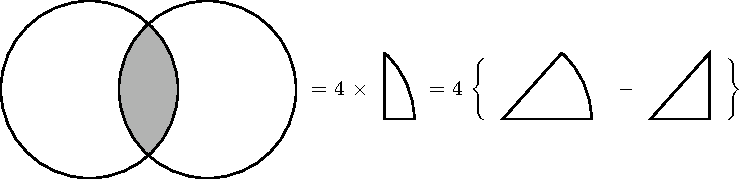
\includegraphics[width = 0.8\textwidth]{../figures/autocorrelation/autocorrelation.pdf}
   \caption{Geometric construction for evaluating the autocorrelations. We need
     to integrate over the overlapping region of two circles with radius $\nu_o$
     and distance $\nu$ between their centers. The region is given by four times
     the difference in area between a sector of angle
     $\arccos\left(\frac{\nu}{2\nu_o}\right)$ and a triangle with base $\nu/2$
     and hypotenuse $\nu_o$.}
   \label{fig:geometry}
 \end{figure}

 To evaluate $A_2(\nu)$ we could follow the same steps, but we will reach a dead
 end because there is no Hankel transform identity for
 $\mathcal{H}_{n-1}\left\{\frac{J_{n+1}(2\pi\nu_o r_o)}{2\pi\nu_o r_o}\right\}$.
 Instead, we rewrite $A_2(\nu)$ as
\begin{align}
  A_2(\nu) = \frac{2}{\pi}\mathcal{F}_2\left\{\left[\frac{J_2(2\pi\nu_o r_o)}{2\pi\nu_o r_o}\right]^2\right\} = \frac{2}{\pi}\left[\mathcal{F}_2\left\{\left[\frac{J_2(2\pi\nu_o r_o)}{2\pi\nu_o r_o}\cos\phi_{\nu}\right]^2\right\} + \mathcal{F}_2\left\{\left[\frac{J_2(2\pi\nu_o r_o)}{2\pi\nu_o r_o}\sin\phi_{\nu}\right]^2\right\}\right].
\end{align}
Applying the autocorrelation theorem gives
\begin{align}
  A_2(\nu) = \frac{2}{\pi}\Bigg[&\mathcal{F}_2\left\{\frac{J_2(2\pi\nu_o r_o)}{2\pi\nu_o r_o}\cos\phi_{\nu}\right\} \star_2 \mathcal{F}_2\left\{\frac{J_2(2\pi\nu_o r_o)}{2\pi\nu_o r_o}\cos\phi_{\nu}\right\} + \nonumber\\ &\mathcal{F}_2\left\{\frac{J_2(2\pi\nu_o r_o)}{2\pi\nu_o r_o}\sin\phi_{\nu}\right\} \star_2 \mathcal{F}_2\left\{\frac{J_2(2\pi\nu_o r_o)}{2\pi\nu_o r_o}\sin\phi_{\nu}\right\}\Bigg].
\end{align}
After converting the Fourier transforms to Hankel transforms with the identities
\begin{align}
  \mathcal{F}_2\left\{f(r)\cos(\phi)\right\} &= -i\cos\phi_{\nu}\mathcal{H}_1\left\{f(r)\right\},\\
  \mathcal{F}_2\left\{f(r)\sin(\phi)\right\} &= -i\sin\phi_{\nu}\mathcal{H}_1\left\{f(r)\right\},
\end{align}
and evaluating the Hankel transforms with Eq. \ref{eq:identity}, we find that
\begin{align}
  A_2(\nu) = -\frac{2}{\pi\nu_o^4}\left\{\left[\nu_x\Pi\left(\frac{\nu}{\nu_o}\right) \star_2 \nu_x\Pi\left(\frac{\nu}{\nu_o}\right)\right] + \left[\nu_y\Pi\left(\frac{\nu}{\nu_o}\right) \star_2 \nu_y\Pi\left(\frac{\nu}{\nu_o}\right)\right]\right\}. \label{eq:long}
\end{align}
Eq. \ref{eq:long} contains two autocorrelations that require us to find the
weighted overlap of two circles. Neither of these autocorrelations are
rotationally symmetric, but their sum must be rotationally symmetric. With this
symmetry in mind, we recognize that the first autocorrelation is largest for
shifts along the $x$ direction and smallest for shifts along the $y$ direction
with a smooth $\cos^2\phi_{\nu}$ weighting between the two extremes. The same is
true for the second autocorrelations except the $x$ and $y$ axes are exchanged
and there is a $\sin^2\phi_{\nu}$ weighting between the two extremes. Therefore,
we can rewrite Eq. \ref{eq:long} as
\begin{align}
  A_2(\nu) = -\frac{2}{\pi\nu_o^4}\Bigg\{&\left[\nu_x\Pi\left(\frac{\nu}{\nu_o}\right) \star_2^x \nu_x\Pi\left(\frac{\nu}{\nu_o}\right)\right]\cos^2\phi_\nu + \left[\nu_x\Pi\left(\frac{\nu}{\nu_o}\right) \star_2^y \nu_x\Pi\left(\frac{\nu}{\nu_o}\right)\right]\sin^2\phi_\nu + \nonumber\\ &\left[\nu_y\Pi\left(\frac{\nu}{\nu_o}\right) \star_2^x \nu_y\Pi\left(\frac{\nu}{\nu_o}\right)\right]\cos^2\phi_\nu + \left[\nu_y\Pi\left(\frac{\nu}{\nu_o}\right) \star_2^y \nu_y\Pi\left(\frac{\nu}{\nu_o}\right)\right]\sin^2\phi_\nu\Bigg\}. \label{eq:long3}
\end{align}
where $\star_2^x$ denotes a two-dimensional autocorrelation for shifts along
the $x$ direction. We can use the following pair of identities
\begin{align}
  \nu_x\Pi\left(\frac{\nu}{\nu_o}\right) \star_2^x \nu_x\Pi\left(\frac{\nu}{\nu_o}\right) = \nu_y\Pi\left(\frac{\nu}{\nu_o}\right) \star_2^y \nu_y\Pi\left(\frac{\nu}{\nu_o}\right),\\
  \nu_x\Pi\left(\frac{\nu}{\nu_o}\right) \star_2^y \nu_x\Pi\left(\frac{\nu}{\nu_o}\right) = \nu_y\Pi\left(\frac{\nu}{\nu_o}\right) \star_2^x \nu_y\Pi\left(\frac{\nu}{\nu_o}\right),
\end{align}
to simplify Eq. \ref{eq:long3} to
\begin{align}
  A_2(\nu) = -\frac{2}{\pi\nu_o^4}\Bigg\{&\left[\nu_x\Pi\left(\frac{\nu}{\nu_o}\right) \star_2^x \nu_x\Pi\left(\frac{\nu}{\nu_o}\right)\right] + \left[\nu_x\Pi\left(\frac{\nu}{\nu_o}\right) \star_2^y \nu_x\Pi\left(\frac{\nu}{\nu_o}\right)\right]\Bigg\}. \label{eq:long4}
\end{align}
First we evaluate the autocorrelation for shifts along the $x$ axis
\begin{align}
  &= -\frac{2}{\pi\nu_o^4}\left[\nu_x\Pi\left(\frac{\nu}{\nu_o}\right) \star_2^x \nu_x\Pi\left(\frac{\nu}{\nu_o}\right)\right]\\
  &= -\frac{8}{\pi\nu_o^4}\Bigg[\int_0^{\nu_o}\tau d\tau\int_0^{\cos^{-1}\left(\frac{\nu}{2\nu_o}\right)}d\phi_{\tau}(-\tau^2\cos^2\phi_{\tau} + \nu\tau\cos\phi_{\tau})\\ &\hspace{5em}- \int_{0}^{\nu/2}d\tau_x\int_0^{\tau_x\frac{2\nu_o}{\nu}\sqrt{1 - \left(\frac{\nu}{2\nu_o}\right)^2}}d\tau_y(-\tau_x^2 + \nu\tau_x)\Bigg]\Pi\left(\frac{\nu}{2\nu_o}\right).
\end{align}
For the first inner integral we make use of the following identities
\begin{align}
  \int_0^{\cos^{-1}z}d\phi\cos^2\phi &= \frac{1}{2}z\sqrt{1 - z^2} + \frac{1}{2}\cos^{-1}z,\\
  \int_0^{\cos^{-1}z}d\phi\cos\phi &= \sqrt{1 - z^2},
\end{align}
which results in
\begin{align}
  &= -\frac{8}{\pi\nu_o^{4}}\Bigg[\int_0^{\nu_o}d\tau\frac{-\tau^3}{2}\left(\frac{\nu}{2\nu_o}\sqrt{1 - \left(\frac{\nu}{2\nu_o}\right)^2} + \cos^{-1}\left(\frac{\nu}{2\nu_o}\right)\right) + \nu\tau^2\sqrt{1 - \left(\frac{\nu}{2\nu_o}\right)^2}\nonumber\\ &\hspace{5em}\int_{0}^{\nu/2}d\tau_x\int_0^{\tau_x\frac{2\nu_o}{\nu}\sqrt{1 - \left(\frac{\nu}{2\nu_o}\right)^2}}d\tau_y(-\tau_x^2 + \nu\tau_x)\Bigg]\Pi\left(\frac{\nu}{2\nu_o}\right),\\
  &=  -\frac{8}{\pi\nu_o^4}\Bigg[\frac{-\nu_o^4}{8}\left(\frac{\nu}{2\nu_o}\sqrt{1 - \left(\frac{\nu}{2\nu_o}\right)^2} + \arccos\left(\frac{\nu}{2\nu_o}\right) \right) + \frac{2\nu_o^4}{3}\frac{\nu}{2\nu_o}\sqrt{1 - \left(\frac{\nu}{2\nu_o}\right)}\nonumber \\ &\hspace{5em} - \frac{5\nu^2\nu_o^2}{48}\frac{\nu}{2\nu_o}\sqrt{1 - \left(\frac{\nu}{2\nu_o}\right)^2}\Bigg]\Pi\left(\frac{\nu}{2\nu_o}\right),\\
  &=  \frac{1}{\pi}\Bigg[\left(\frac{\nu}{2\nu_o}\sqrt{1 - \left(\frac{\nu}{2\nu_o}\right)^2} + \arccos\left(\frac{\nu}{2\nu_o}\right) \right) - \frac{16}{3}\frac{\nu}{2\nu_o}\sqrt{1 - \left(\frac{\nu}{2\nu_o}\right)}\nonumber \\ &\hspace{5em} + \frac{5\nu^2}{6\nu_o^2}\frac{\nu}{2\nu_o}\sqrt{1 - \left(\frac{\nu}{2\nu_o}\right)^2}\Bigg]\Pi\left(\frac{\nu}{2\nu_o}\right),\\
  &= \frac{1}{\pi}\left[\arccos\left(\frac{\nu}{2\nu_o}\right) - \left(\frac{13}{3} - \frac{5\nu^2}{6\nu_o^2}\right)\frac{\nu}{2\nu_o} \sqrt{1 - \left(\frac{\nu}{2\nu_o}\right)^2}\right]\Pi\left(\frac{\nu}{2\nu_o}\right),\\
  &= \frac{1}{\pi}\left[\arccos\left(\frac{\nu}{2\nu_o}\right) - \frac{1}{3}\left[13 - 10\left(\frac{\nu}{2\nu_o}\right)^2\right]\frac{\nu}{2\nu_o} \sqrt{1 - \left(\frac{\nu}{2\nu_o}\right)^2}\right]\Pi\left(\frac{\nu}{2\nu_o}\right).\label{eq:auto1}
\end{align}
Next we evaluate the autocorrelation for shifts along the $y$ axis
\begin{align}
  &\frac{-2}{\pi\nu_0^4}\left\{\left[\nu_x\, \Pi\left(\frac{\nu}{\nu_o}\right)\right] \star_2^y \left[\nu_x\, \Pi\left(\frac{\nu}{\nu_o}\right)\right]\right\} = \\
  &=  \frac{-8}{\pi\nu_o^4}\Bigg[\int\limits_0^{\nu_o} d\tau\, \tau \int\limits_0^{\cos^{-1}\left(\frac{\nu}{2\nu_o}\right)}d\phi_{\tau}(-\tau^2\sin^2\phi_{\tau}) - \int\limits_0^{\nu/2}d\tau_x \int\limits_0^{\tau_x \frac{2\nu_o}{\nu}\sqrt{1 - \left(\frac{\nu}{2\nu_o}\right)^2}}d\tau_y(-\tau_y^2)\Bigg]\Pi\left(\frac{\nu}{2\nu_o}\right).
\end{align}
For the first inner integral we make use of
\begin{align}
  \int\limits_0^{\cos^{-1}z} d\phi \sin^2\phi &= -\frac{1}{2}z\sqrt{1 - z^2} + \frac{1}{2}\cos^{-1}(z).
\end{align}
This results in
\begin{align}
  &=\frac{-8}{\pi\nu_o^4}\Bigg[\int\limits_0^{\nu_o} d\tau\, \frac{-\tau^3}{2}\left(\frac{-\nu}{2\nu_o}\sqrt{1 - \left(\frac{\nu}{2\nu_o}\right)^2} + \cos^{-1}\left(\frac{\nu}{2a}\right)\right) - \int\limits_0^{\nu/2}d\tau_x \frac{-\tau_x^3}{3}\left(\frac{2 \nu_o}{\nu}\sqrt{1 - \left(\frac{\nu}{2\nu_o}\right)^2}\right)^3\Bigg]\Pi\left(\frac{\nu}{2\nu_o}\right),\\
  &=  \frac{-8}{\pi\nu_o^4}\Bigg[\frac{-\nu_o^4}{8}\left(\frac{-\nu}{2\nu_o}\sqrt{1 - \left(\frac{\nu}{2\nu_o}\right)^2} + \cos^{-1}\left(\frac{\nu}{2\nu_o}\right) \right) + \frac{\nu_o^4}{12}\frac{\nu}{2\nu_o}\sqrt[3]{1 - \left(\frac{\nu}{2\nu_o}\right)^2}\Bigg]\Pi\left(\frac{\nu}{2\nu_o}\right),\\
  &=  \frac{1}{\pi}\Bigg[\cos^{-1}\left(\frac{\nu}{2\nu_o}\right) - \frac{1}{3}\left[5 - 2\left(\frac{\nu}{2\nu_o}\right)^2\right]\frac{\nu}{2\nu_o}\sqrt{1 - \left(\frac{\nu}{2\nu_o}\right)^2}\Bigg]\Pi\left(\frac{\nu}{2\nu_o}\right). \label{eq:auto2}
\end{align}
Taking the sum of Eqs. \ref{eq:auto1} and \ref{eq:auto2} gives the final result
\begin{align}
  A_2(\nu) = \frac{2}{\pi}\Bigg\{\cos^{-1}\left(\frac{\nu}{2\nu_o}\right) - \left[3 - 2\left(\frac{\nu}{2\nu_o}\right)^2\right]\frac{\nu}{2\nu_o}\sqrt{1 - \left(\frac{\nu}{2\nu_o}\right)^2}\Bigg\}\Pi\left(\frac{\nu}{2\nu_o}\right). 
\end{align}

\end{document}
